\begin{center}
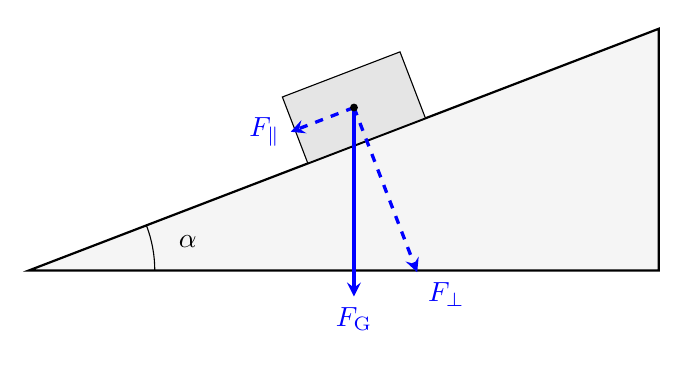
\begin{tikzpicture}[>=stealth]
 \draw[thick, fill=gray!8] (0,0) -- (8.00,0) -- (8.00,3.07) -- cycle;
 \draw (1.6,0) arc (0:21:1.6);
 \node at (2.02,0.37) {$\alpha$};
 \begin{scope}[shift={(4.29,1.65)}, rotate=21]
  \draw[fill=gray!20] (-0.8,0) rectangle (0.8,0.9);
 \end{scope}
 \draw[->, very thick, blue] (4.13,2.07) -- ++(-90.00:2.40) node[anchor=north] {$F_\mathrm{G}$};
 \draw[->, very thick, blue, dashed] (4.13,2.07) -- ++(-69.00:2.24) node[anchor=north west] {$F_\perp$};
 \draw[->, very thick, blue, dashed] (4.13,2.07) -- ++(201.00:0.86) node[anchor=east] {$F_\parallel$};
 \fill (4.13,2.07) circle (0.05);
\end{tikzpicture}
\end{center}

Die Gewichtskraft $F_\mathrm{G} = m\,g = \FGe$ wird in eine Komponente senkrecht und eine parallel zur Rampe zerlegt. Der Winkel zwischen $F_\mathrm{G}$ und $F_\perp$ ist gleich dem Neigungswinkel $\alpha = \wiO$:
\begin{align}
 F_\perp &= \FskF = \mKi\cdot\gE\cdot\cos\left(\wiO\right) = \Fsk \approx \result{\FskP{0}{2}} \\
 F_\parallel &= \FpaF = \mKi\cdot\gE\cdot\sin\left(\wiO\right) = \Fpa \approx \result{\FpaP{0}{2}}
\end{align}
